\documentclass[12pt]{article}

\usepackage[utf8]{inputenc}
\usepackage[T1]{fontenc}
\usepackage[brazilian]{babel}
\usepackage{geometry}
\usepackage{hyperref}
\usepackage{graphicx}
\usepackage{subcaption}
\usepackage{xcolor}
\usepackage{titlesec}
\usepackage{enumitem}
\usepackage{booktabs}
\usepackage{float}
\usepackage{array}
\usepackage{tikz}
\usetikzlibrary{arrows.meta, positioning, shapes.geometric}

\geometry{left=1.8cm, right=1.8cm, top=2cm, bottom=2cm}
\titlespacing*{\section}{0pt}{1.2ex plus 1ex minus .2ex}{0.8ex plus .2ex}
\titlespacing*{\subsection}{0pt}{1ex plus 1ex minus .2ex}{0.6ex plus .2ex}

\graphicspath{{figuras/}}

\title{Relat\'orio Final: Minera\c{c}\~ao de Regras de Associa\c{c}\~ao \\ em Acidentes em Rodovias Federais (MG)}

\author{Erik Roberto Reis Neves \\ Gabriel Campos Prudente \\ Felipe Silva Fraga Damasceno}

\date{Junho de 2026}

\begin{document}

\maketitle

\begin{abstract}
Este relat\'orio apresenta um estudo completo de Minera\c{c}\~ao de Dados sobre acidentes em rodovias federais registrados pela Pol\'icia Rodovi\'aria Federal (PRF), com recorte geogr\'afico em Minas Gerais (MG) e janela temporal multi-ano (2023--2026). Adotamos o algoritmo FP-Growth para extrair regras de associa\c{c}\~ao do tipo \textit{contexto} $\rightarrow$ \textit{desfecho\_Fatal}, evitando tautologias entre vari\'aveis de gravidade. Sobre 26.899 ocorr\^encias com v\'itimas, identificamos 76 regras n\~ao triviais (lift m\'aximo 5,44) e 87 padr\~oes temporalmente est\'aveis. Operacionalizamos as diretrizes de IA respons\'avel \textbf{Explicabilidade} e \textbf{Monitoramento e Avalia\c{c}\~ao} na sele\c{c}\~ao, tradu\c{c}\~ao e valida\c{c}\~ao temporal das regras. Os resultados indicam combina\c{c}\~oes recorrentes envolvendo colis\~oes frontais, trechos rurais, pista simples e condi\c{c}\~oes noturnas associadas a desfechos fatais, com implica\c{c}\~oes para preven\c{c}\~ao vi\'aria, ressalvada a distin\c{c}\~ao entre associa\c{c}\~ao estat\'istica e causalidade.
\end{abstract}

\section{Introdu\c{c}\~ao}

Os acidentes de tr\^ansito em rodovias federais constituem um problema de sa\'ude p\'ublica e infraestrutura no Brasil, com perdas humanas e custos socioecon\^omicos elevados. A Pol\'icia Rodovi\'aria Federal (PRF) registra sistematicamente essas ocorr\^encias, produzindo bases de dados ricas em vari\'aveis temporais, ambientais, vi\'arias e de consequ\^encia. An\'alises univariadas ou puramente descritivas s\~ao insuficientes para capturar a intera\c{c}\~ao simult\^anea de m\'ultiplos fatores de risco; a gravidade dos acidentes emerge, em geral, da \textbf{coocorr\^encia} de condi\c{c}\~oes contextuais, e n\~ao de vari\'aveis isoladas.

\subsection{Objetivos}

O objetivo geral deste projeto \'e desenvolver um estudo de Minera\c{c}\~ao de Dados sobre acidentes rodovi\'arios federais, identificando \textbf{padr\~oes ocultos e regras de associa\c{c}\~ao estatisticamente relevantes} associadas \`a severidade dos acidentes. Os objetivos espec\'ificos s\~ao:
\begin{enumerate}[leftmargin=*]
    \item Identificar itemsets frequentes que caracterizem cen\'arios de risco em MG, com representa\c{c}\~ao transacional one-hot.
    \item Gerar regras \textit{contexto} $\rightarrow$ \textit{Fatal} com m\'etricas de suporte, confian\c{c}a, lift e conviction, priorizando padr\~oes interpret\'aveis e n\~ao redundantes.
    \item Investigar heterogeneidades estruturais por estrato de \textit{uso do solo} (urbano vs.\ rural).
    \item Operacionalizar as diretrizes de IA respons\'avel \textbf{Explicabilidade} e \textbf{Monitoramento e Avalia\c{c}\~ao}.
\end{enumerate}

\subsection{Problema Investigado}

Buscamos regras de associa\c{c}\~ao \textbf{n\~ao triviais} que relacionem combina\c{c}\~oes de fatores contextuais --- ambientais, temporais e vi\'arios --- \`a ocorr\^encia de acidentes com desfecho fatal entre ocorr\^encias \textbf{com v\'itimas}. O desafio n\~ao \'e apenas encontrar padr\~oes frequentes, mas extrair regras simultaneamente \textbf{interpret\'aveis, relevantes e n\~ao redundantes}, evitando tautologias (por exemplo, regras que apenas reproduzem a classifica\c{c}\~ao oficial de gravidade).

\section{Trabalhos Relacionados}

\subsection{Minera\c{c}\~ao de Padr\~oes Frequentes e Regras de Associa\c{c}\~ao}

Agrawal e Srikant \cite{agrawal1994} formalizaram a minera\c{c}\~ao de regras de associa\c{c}\~ao sobre bases transacionais, introduzindo suporte e confian\c{c}a como m\'etricas centrais. Han \textit{et al.} \cite{han2000} propuseram o algoritmo FP-Growth, que compacta transa\c{c}\~oes em uma FP-Tree e evita a gera\c{c}\~ao expl\'icita de candidatos, sendo adequado a bases de alta dimensionalidade. Zaki e Meira Jr.\ \cite{zaki2020} sistematizam m\'etricas complementares --- lift, leverage e conviction --- para filtrar associa\c{c}\~oes esp\'urias e priorizar padr\~oes informativos.

\subsection{Metodologia CRISP-DM}

Wirth e Hipp \cite{wirth2000} prop\~oem o CRISP-DM como processo padr\~ao para projetos de minera\c{c}\~ao de dados, estruturando o trabalho em fases iterativas: compreens\~ao do neg\'ocio e dos dados, prepara\c{c}\~ao, modelagem, avalia\c{c}\~ao e deployment. Adotamos essa estrutura para organizar notebooks reprodut\'iveis e um pipeline em \texttt{src/}.

\subsection{Dados Abertos da PRF}

A PRF disponibiliza publicamente bases consolidadas de acidentes em rodovias federais \cite{prf2026}, com vari\'aveis temporais, espaciais, ambientais e de gravidade. Estudos descritivos s\~ao comuns, mas a aplica\c{c}\~ao sistem\'atica de regras de associa\c{c}\~ao multivariadas sobre recortes regionais multi-ano permanece pouco explorada.

\section{Metodologia}

O projeto seguiu o framework CRISP-DM (Figura~\ref{fig:pipeline}), com redesenho metodol\'ogico \textbf{Pacote~A}: minera\c{c}\~ao restrita a regras \textit{contexto} $\rightarrow$ \textit{desfecho\_Fatal}, sem incluir vari\'aveis tautol\'ogicas de gravidade nos antecedentes.

\begin{figure}[H]
    \centering
    \begin{tikzpicture}[
        node distance=0.55cm and 0.35cm,
        box/.style={rectangle, draw, rounded corners, minimum width=2.6cm, minimum height=0.65cm, align=center, font=\small},
        arrow/.style={-{Stealth[length=2mm]}, thick}
    ]
        \node[box] (d1) {Dados PRF\\(2023--2026, MG)};
        \node[box, below=of d1] (d2) {EDA e\\qualidade};
        \node[box, below=of d2] (d3) {Prepara\c{c}\~ao\\Pacote A};
        \node[box, below=of d3] (d4) {FP-Growth\\restrito};
        \node[box, below left=0.6cm and -0.2cm of d4] (d5) {Estabilidade\\temporal};
        \node[box, below right=0.6cm and -0.2cm of d4] (d6) {Estratos\\urbano/rural};
        \node[box, below=1.1cm of d4] (d7) {Avalia\c{c}\~ao e\\visualiza\c{c}\~ao};
        \draw[arrow] (d1) -- (d2);
        \draw[arrow] (d2) -- (d3);
        \draw[arrow] (d3) -- (d4);
        \draw[arrow] (d4) -- (d5);
        \draw[arrow] (d4) -- (d6);
        \draw[arrow] (d5) -- (d7);
        \draw[arrow] (d6) -- (d7);
    \end{tikzpicture}
    \caption{Pipeline CRISP-DM implementado (Pacote A).}
    \label{fig:pipeline}
\end{figure}

\subsection{Dados e Recorte}

Utilizamos os CSVs \textit{agrupados por ocorr\^encia} da PRF (\texttt{datatran2023.csv}--\texttt{datatran2026.csv}), com separador \texttt{;} e encoding \texttt{latin-1}. Cada registro corresponde a uma ocorr\^encia \'unica. Aplicamos filtro geogr\'afico UF~=~MG, totalizando \textbf{30.858} ocorr\^encias nos quatro anos dispon\'iveis. Restringimos a an\'alise a acidentes \textbf{com v\'itimas} ($n = 26.899$), definindo o alvo bin\'ario \texttt{desfecho} $\in \{$Fatal (7,8\%), Ferido (92,2\%)$\}$.

\subsection{Prepara\c{c}\~ao (Pacote A)}

Selecionamos oito colunas de \textbf{contexto}: \texttt{condicao\_metereologica}, \texttt{tipo\_pista}, \texttt{tracado\_via}, \texttt{uso\_solo}, \texttt{causa\_acidente}, \texttt{tipo\_acidente}, \texttt{fase\_dia} e \texttt{fim\_de\_semana}. Cada ocorr\^encia foi convertida em transa\c{c}\~ao one-hot com prefixo \texttt{ctx\_}, mais o item-alvo \texttt{desfecho\_Fatal} ou \texttt{desfecho\_Ferido}. Itens com frequ\^encia $< 0{,}5\%$ ou $> 99\%$ foram removidos, resultando em 78 itens v\'alidos.

\subsection{Modelagem: FP-Growth Restrito}

O FP-Growth (\texttt{mlxtend}) foi aplicado com \texttt{min\_support = 0{,}005}. As regras foram filtradas para:
\begin{itemize}[leftmargin=*]
    \item consequente exclusivamente \texttt{desfecho\_Fatal};
    \item antecedentes contendo apenas itens \texttt{ctx\_*} (m\'aximo tr\^es itens);
    \item confian\c{c}a $\geq 8\%$, lift $\geq 1{,}05$ e suporte absoluto $\geq 15$ ocorr\^encias;
    \item poda de regras n\~ao minimais e redundantes.
\end{itemize}

\subsection{M\'etricas e Hip\'oteses}

Avaliamos suporte $P(A \cup B)$, confian\c{c}a $P(B \mid A)$, lift (raz\~ao entre confian\c{c}a observada e esperada sob independ\^encia), leverage e conviction. Formulamos cinco hip\'oteses (H1--H5) sobre combina\c{c}\~oes noturnas/rurais, finais de semana, colis\~oes frontais/atropelamentos, clima adverso e heterogeneidade urbano/rural.

\section{Implementa\c{c}\~ao}

A l\'ogica anal\'itica concentra-se em \texttt{src/} (\texttt{data\_loading.py}, \texttt{preparation.py}, \texttt{mining.py}, \texttt{evaluation.py}) e \texttt{scripts/run\_pipeline.py}, que executa o fluxo end-to-end e exporta artefatos em \texttt{outputs/}. Seis notebooks (01--06) documentam setup, EDA, prepara\c{c}\~ao, modelagem, avalia\c{c}\~ao de IA respons\'avel e visualiza\c{c}\~ao. A configura\c{c}\~ao central (\texttt{src/config.py}) garante reprodutibilidade de par\^ametros e caminhos.

\section{Resultados Experimentais}

\subsection{An\'alise Explorat\'oria}

A Tabela~\ref{tab:desfecho} confirma desbalanceamento marcante: apenas 7,8\% dos acidentes com v\'itimas s\~ao fatais. A an\'alise de associa\c{c}\~ao via Cram\'er's~$V$ (Figura~\ref{fig:eda1}) indica que \texttt{tipo\_acidente}, \texttt{causa\_acidente} e \texttt{tracado\_via} s\~ao os contextos mais fortemente associados ao desfecho.

\begin{table}[H]
    \centering
    \caption{Distribui\c{c}\~ao do desfecho entre ocorr\^encias com v\'itimas (MG, 2023--2026).}
    \label{tab:desfecho}
    \begin{tabular}{@{}lrr@{}}
\toprule
\textbf{Desfecho} & \textbf{$n$} & \textbf{\%} \\
\midrule
Ferido & 24.793 & 92.2 \\
Fatal & 2.106 & 7.8 \\
\midrule
Total (com v\'timas) & 26.899 & 100,0 \\
\bottomrule
\end{tabular}
\end{table}

\begin{figure}[H]
    \centering
    \begin{subfigure}[b]{0.48\textwidth}
        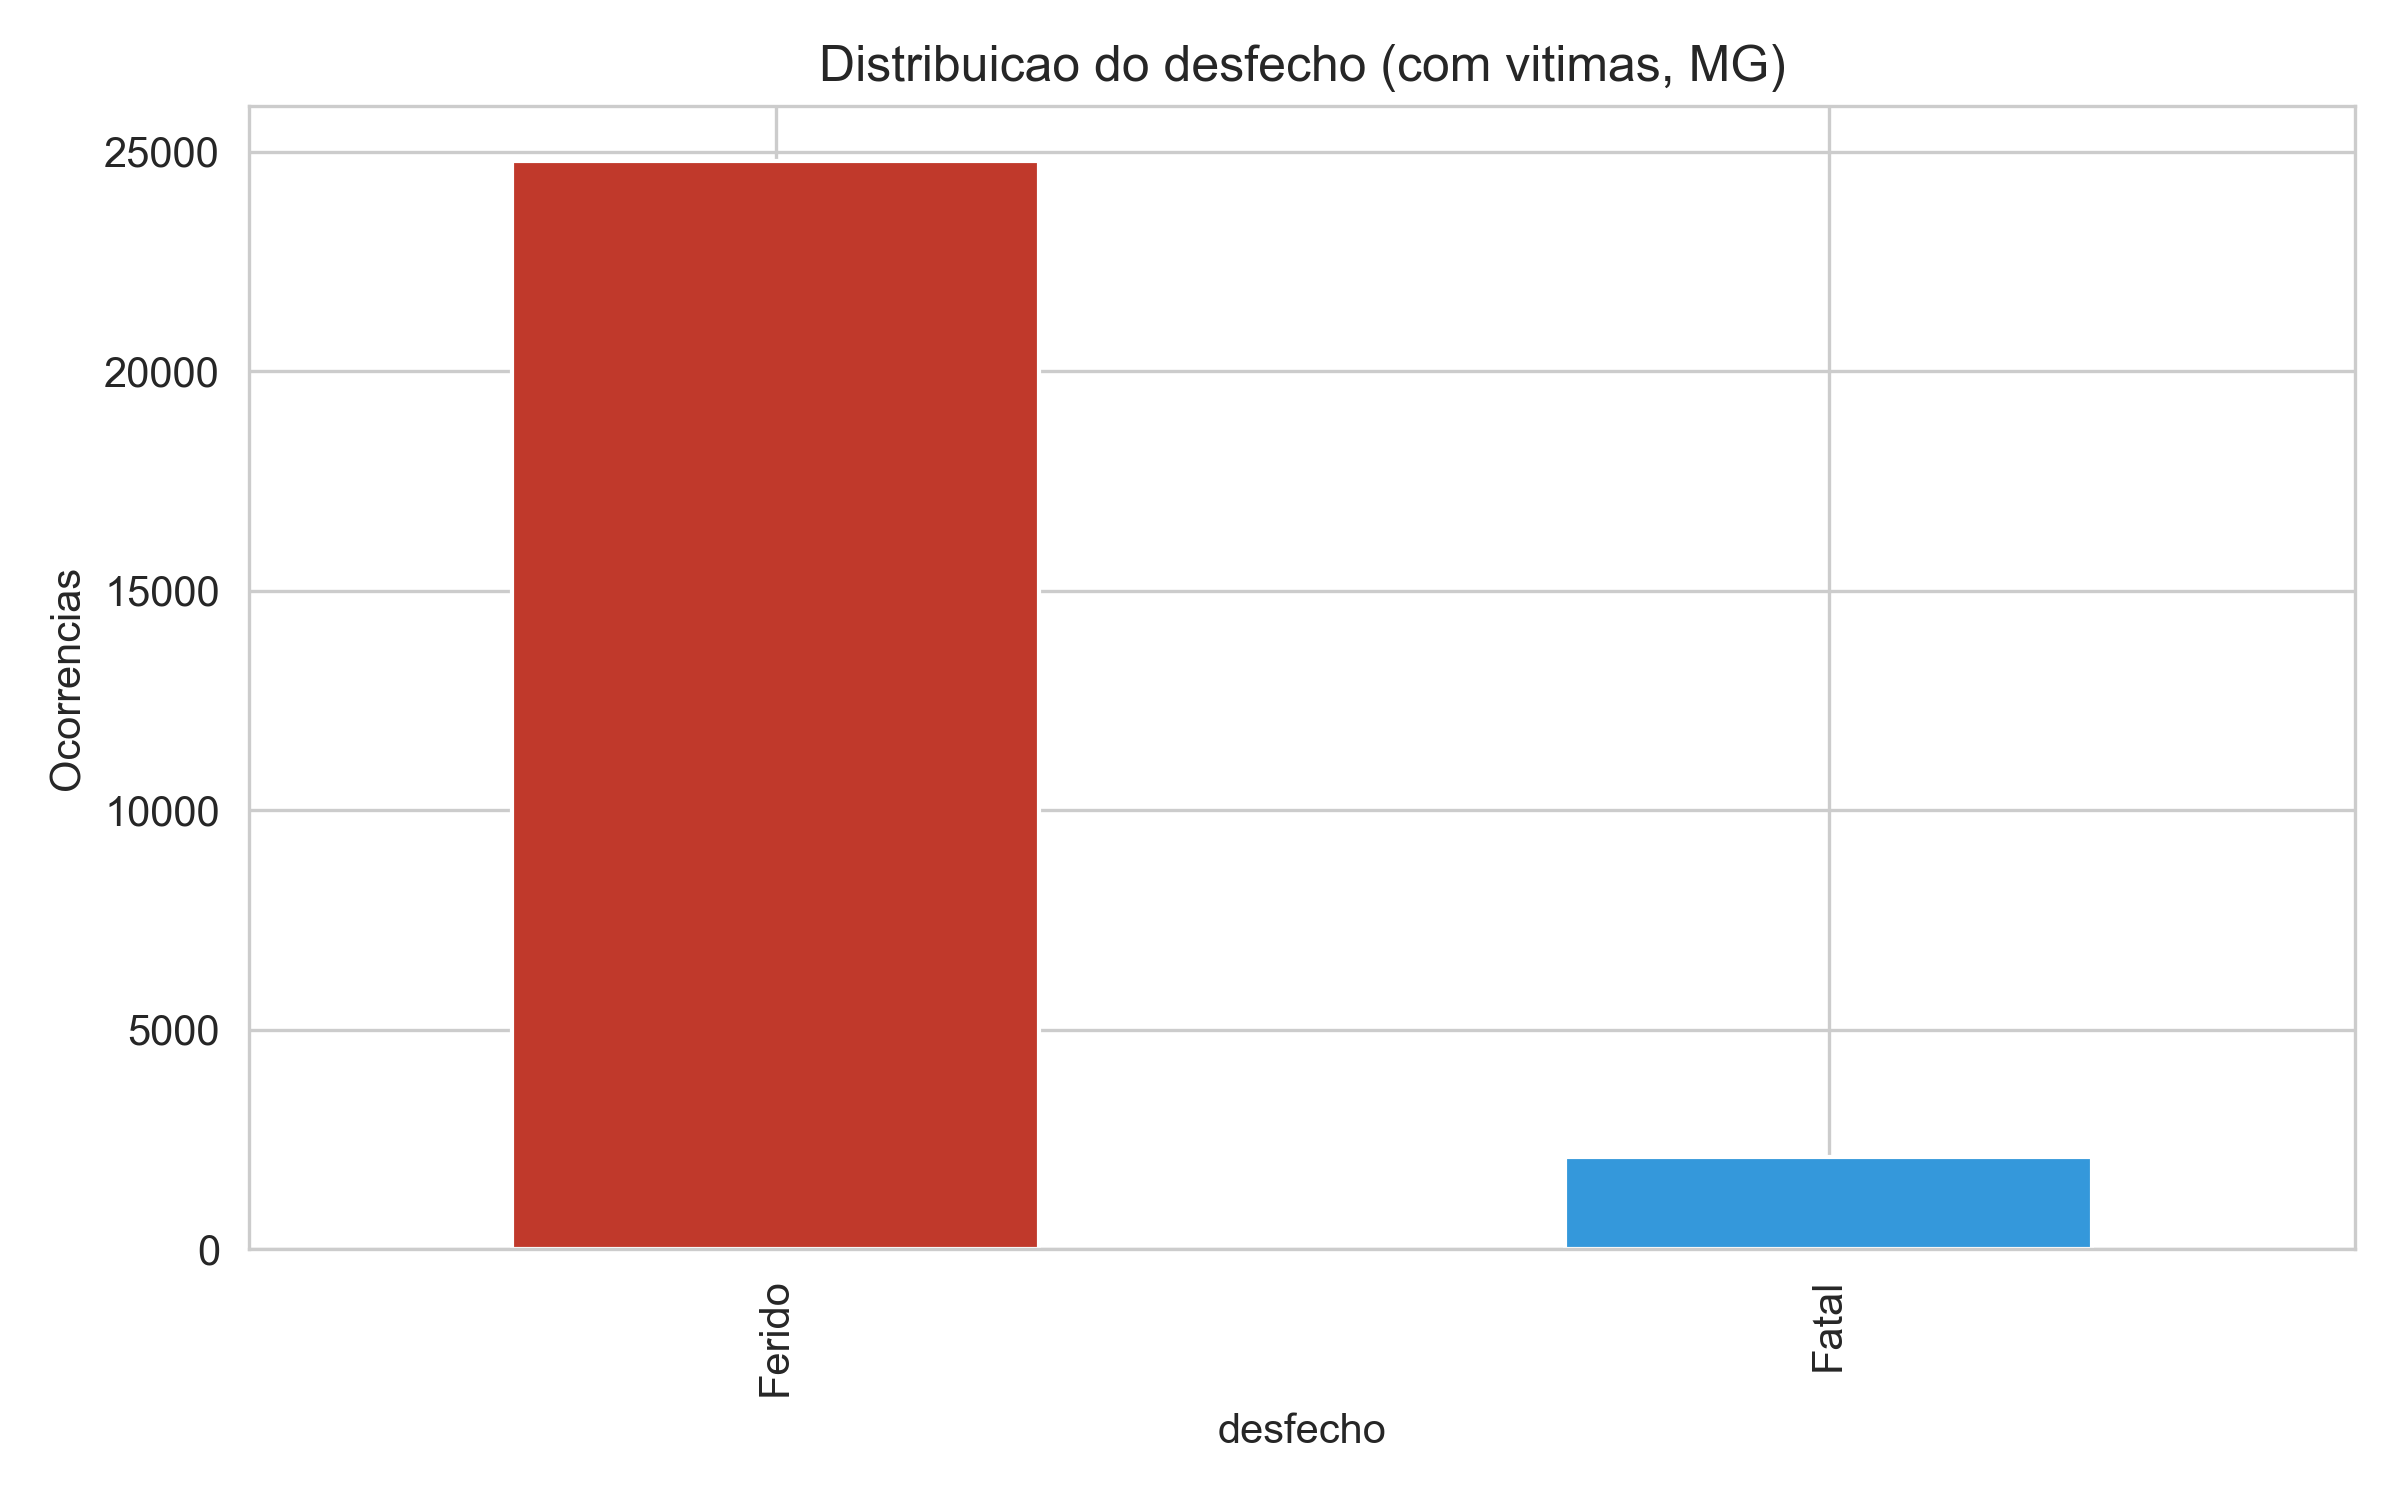
\includegraphics[width=\textwidth]{01_distribuicao_desfecho.png}
        \caption{Distribui\c{c}\~ao do desfecho.}
    \end{subfigure}
    \hfill
    \begin{subfigure}[b]{0.48\textwidth}
        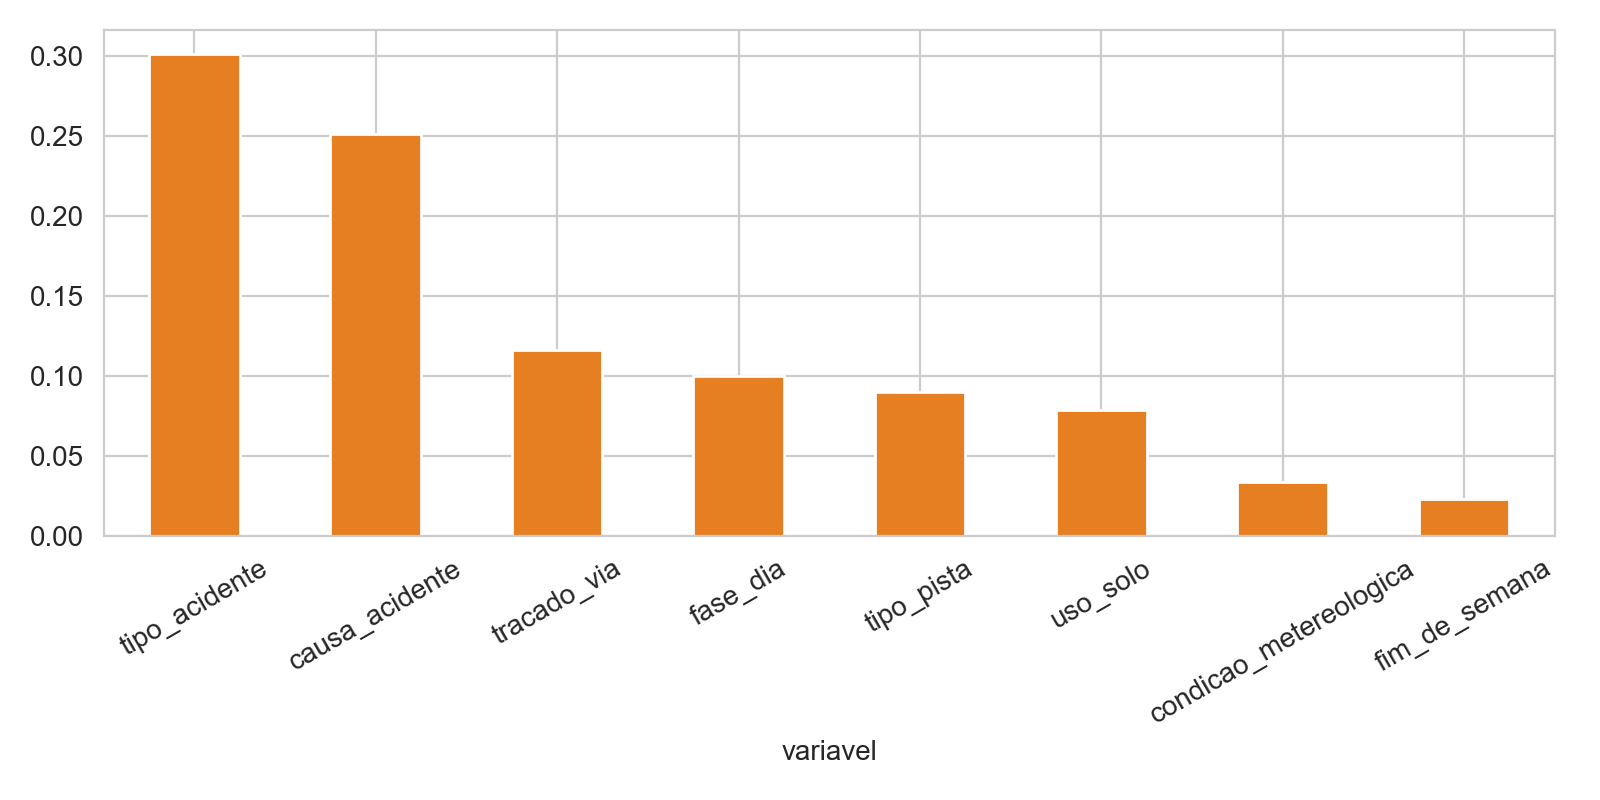
\includegraphics[width=\textwidth]{02_cramers_v_desfecho.png}
        \caption{Cram\'er's $V$ (contexto $\times$ desfecho).}
    \end{subfigure}
    \caption{Resultados explorat\'orios principais.}
    \label{fig:eda1}
\end{figure}

A Figura~\ref{fig:geo} apresenta distribui\c{c}\~ao espacial (amostra de 3.000 pontos) sobre mapa de MG, evidenciando concentra\c{c}\~ao ao longo das BRs e da regi\~ao metropolitana de Belo Horizonte. O perfil temporal (Figura~\ref{fig:tempo}) mostra maior taxa relativa de fatalidade em fases noturnas e varia\c{c}\~ao sazonal entre anos.

\begin{figure}[H]
    \centering
    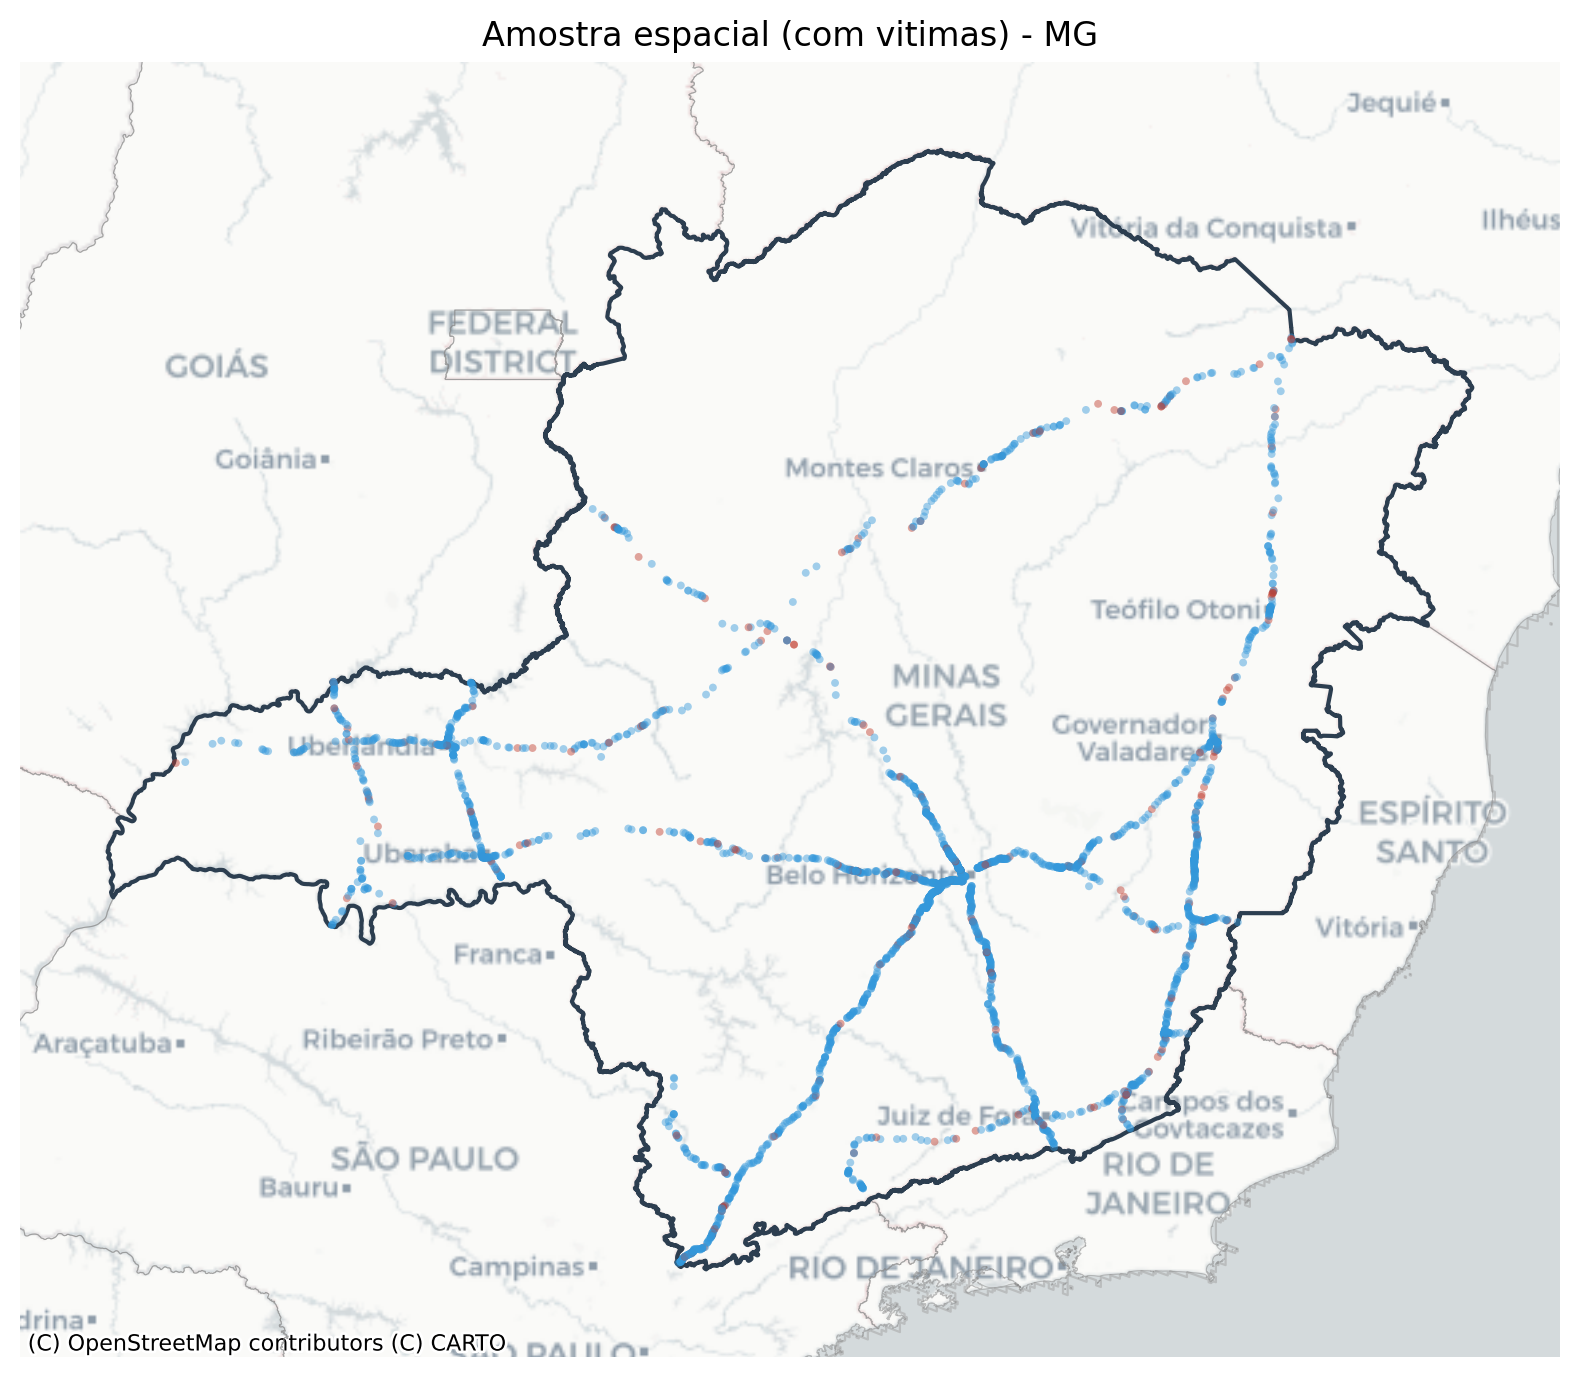
\includegraphics[width=0.72\textwidth]{02_mapa_amostra.png}
    \caption{Amostra espacial de acidentes com v\'itimas em MG (Fatal em vermelho, Ferido em azul).}
    \label{fig:geo}
\end{figure}

\begin{figure}[H]
    \centering
    \begin{subfigure}[b]{0.48\textwidth}
        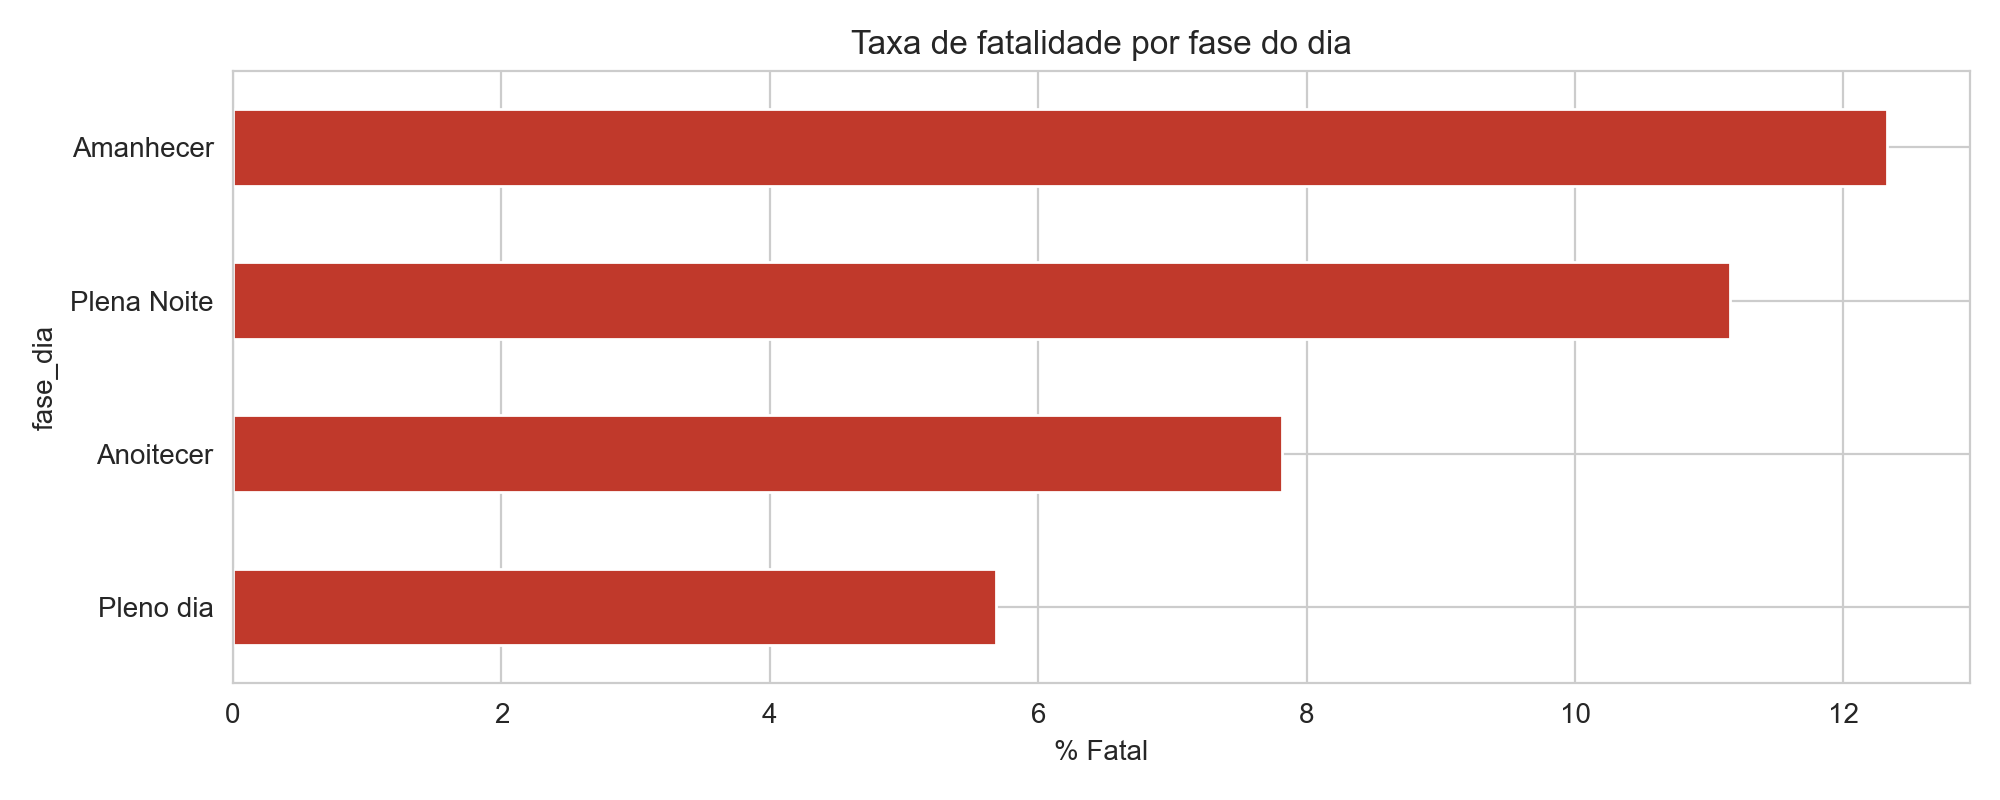
\includegraphics[width=\textwidth]{02_fatal_por_fase_dia.png}
        \caption{Taxa de fatalidade por fase do dia.}
    \end{subfigure}
    \hfill
    \begin{subfigure}[b]{0.48\textwidth}
        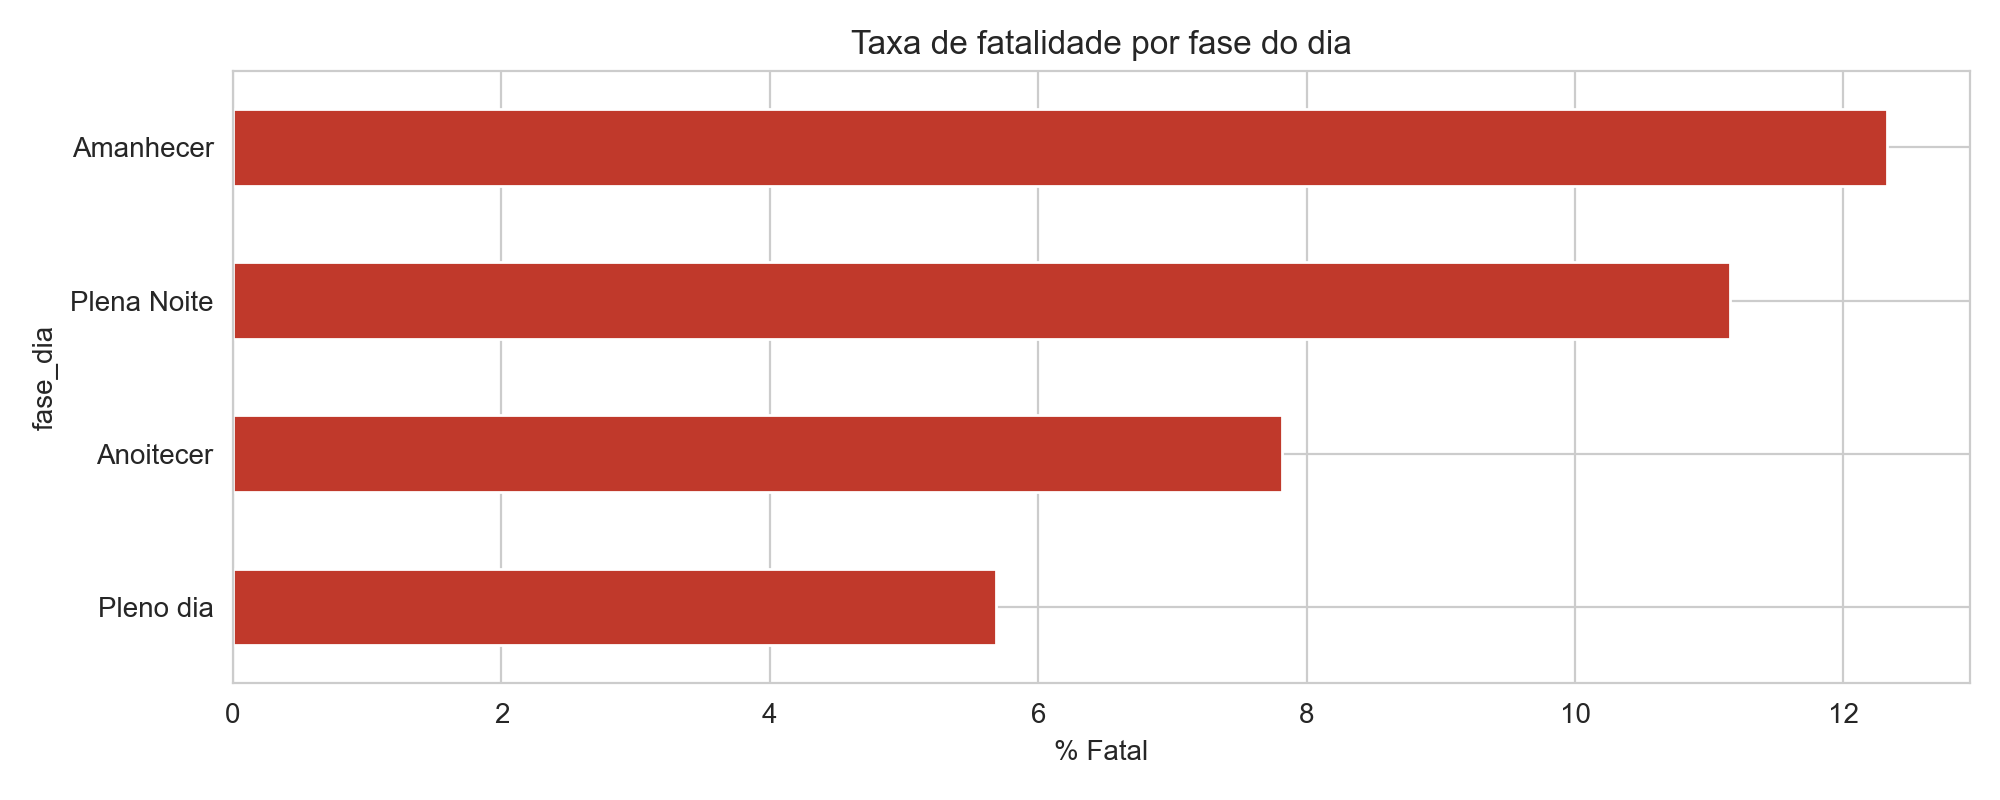
\includegraphics[width=\textwidth]{02_sazonalidade_mensal.png}
        \caption{Sazonalidade mensal por ano.}
    \end{subfigure}
    \caption{Perfil temporal dos acidentes com v\'itimas.}
    \label{fig:tempo}
\end{figure}

\subsection{Regras de Associa\c{c}\~ao}

A minera\c{c}\~ao global produziu \textbf{76 regras} contexto $\rightarrow$ Fatal, com lift m\'aximo de \textbf{5,44} e mediana de \textbf{1,81}. A Tabela~\ref{tab:top} lista as doze regras de maior lift; destacam-se combina\c{c}\~oes envolvendo \textit{Plena Noite + Atropelamento de Pedestre + Zona Rural} (lift 5,44) e \textit{Transitar na contram\~ao + Colis\~ao frontal + Zona Rural} (lift 5,40).

\begin{table}[H]
    \centering
    \caption{Top-12 regras contexto $\rightarrow$ Fatal por lift (base multi-ano).}
    \label{tab:top}
    \small
    \begin{tabular}{@{}p{6.8cm}rrr@{}}
\toprule
\textbf{Antecedente (contexto)} & \textbf{Sup. (\%)} & \textbf{Conf. (\%)} & \textbf{Lift} \\
\midrule
fase dia=Plena Noite; tipo acidente=Atropelamento de Pedestre; uso solo=Não & 0,5 & 42,6 & 5,44 \\
causa acidente=Transitar na contramão; tipo acidente=Colisão frontal; uso solo=Não & 0,7 & 42,3 & 5,40 \\
causa acidente=Transitar na contramão; tipo acidente=Colisão frontal; tipo pista=Simples & 0,8 & 38,9 & 4,97 \\
condicao metereologica=Céu Claro; tipo acidente=Colisão frontal; uso solo=Não & 1,1 & 37,7 & 4,82 \\
fase dia=Plena Noite; tipo acidente=Colisão frontal; uso solo=Não & 0,7 & 37,6 & 4,80 \\
tipo acidente=Colisão frontal; tracado via=Reta; uso solo=Não & 0,9 & 37,5 & 4,79 \\
fim de semana=Sim; tipo acidente=Colisão frontal; uso solo=Não & 0,8 & 37,3 & 4,76 \\
causa acidente=Transitar na contramão; condicao metereologica=Céu Claro; tipo acidente=Colisão frontal & 0,5 & 37,3 & 4,76 \\
causa acidente=Transitar na contramão; tipo acidente=Colisão frontal & 0,8 & 37,1 & 4,73 \\
fase dia=Plena Noite; tipo acidente=Atropelamento de Pedestre & 0,9 & 36,7 & 4,69 \\
tipo acidente=Atropelamento de Pedestre; uso solo=Não & 0,8 & 36,3 & 4,63 \\
tipo acidente=Colisão frontal; tipo pista=Simples; uso solo=Não & 1,9 & 35,8 & 4,57 \\
\bottomrule
\end{tabular}
\end{table}

A Figura~\ref{fig:mining} mostra o scatter suporte$\times$confian\c{c}a (cor = lift) e a contagem de regras por ano. Observa-se que regras de alto lift tendem a apresentar suporte baixo ($< 2\%$), coerente com a raridade de desfechos fatais.

\begin{figure}[H]
    \centering
    \begin{subfigure}[b]{0.48\textwidth}
        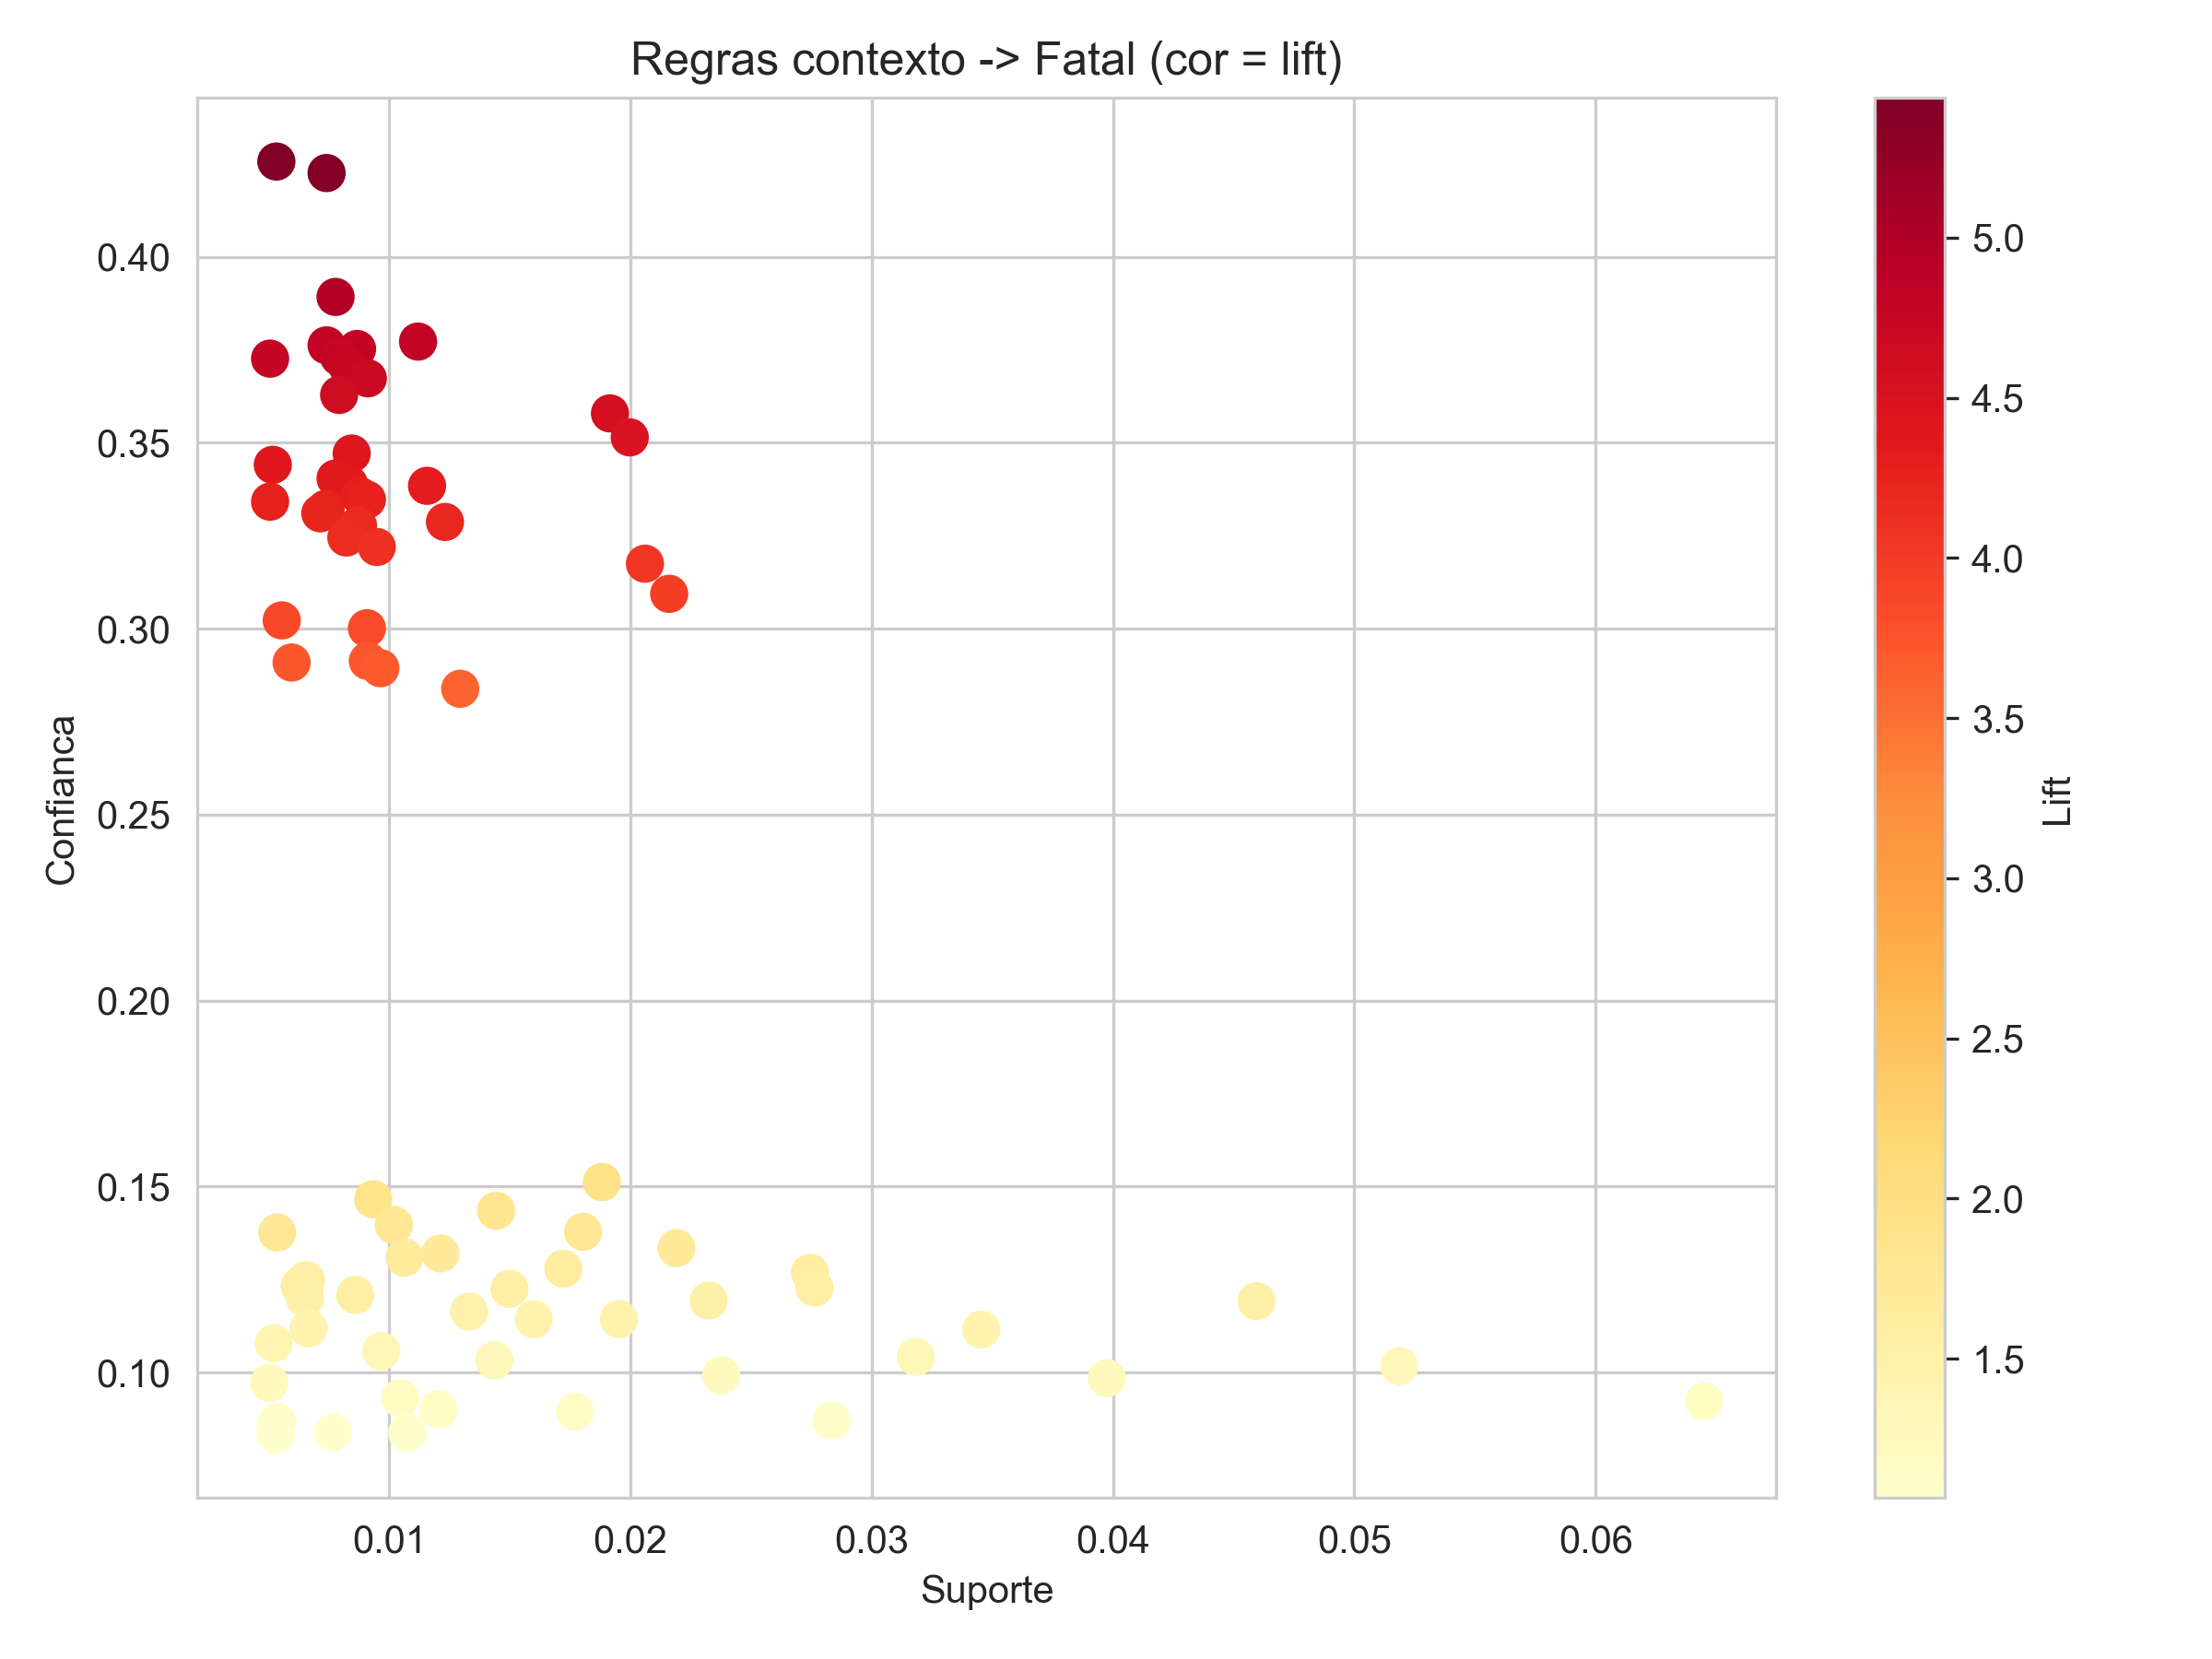
\includegraphics[width=\textwidth]{05_scatter_suporte_confianca_fatal.png}
        \caption{Suporte $\times$ confian\c{c}a (cor = lift).}
    \end{subfigure}
    \hfill
    \begin{subfigure}[b]{0.48\textwidth}
        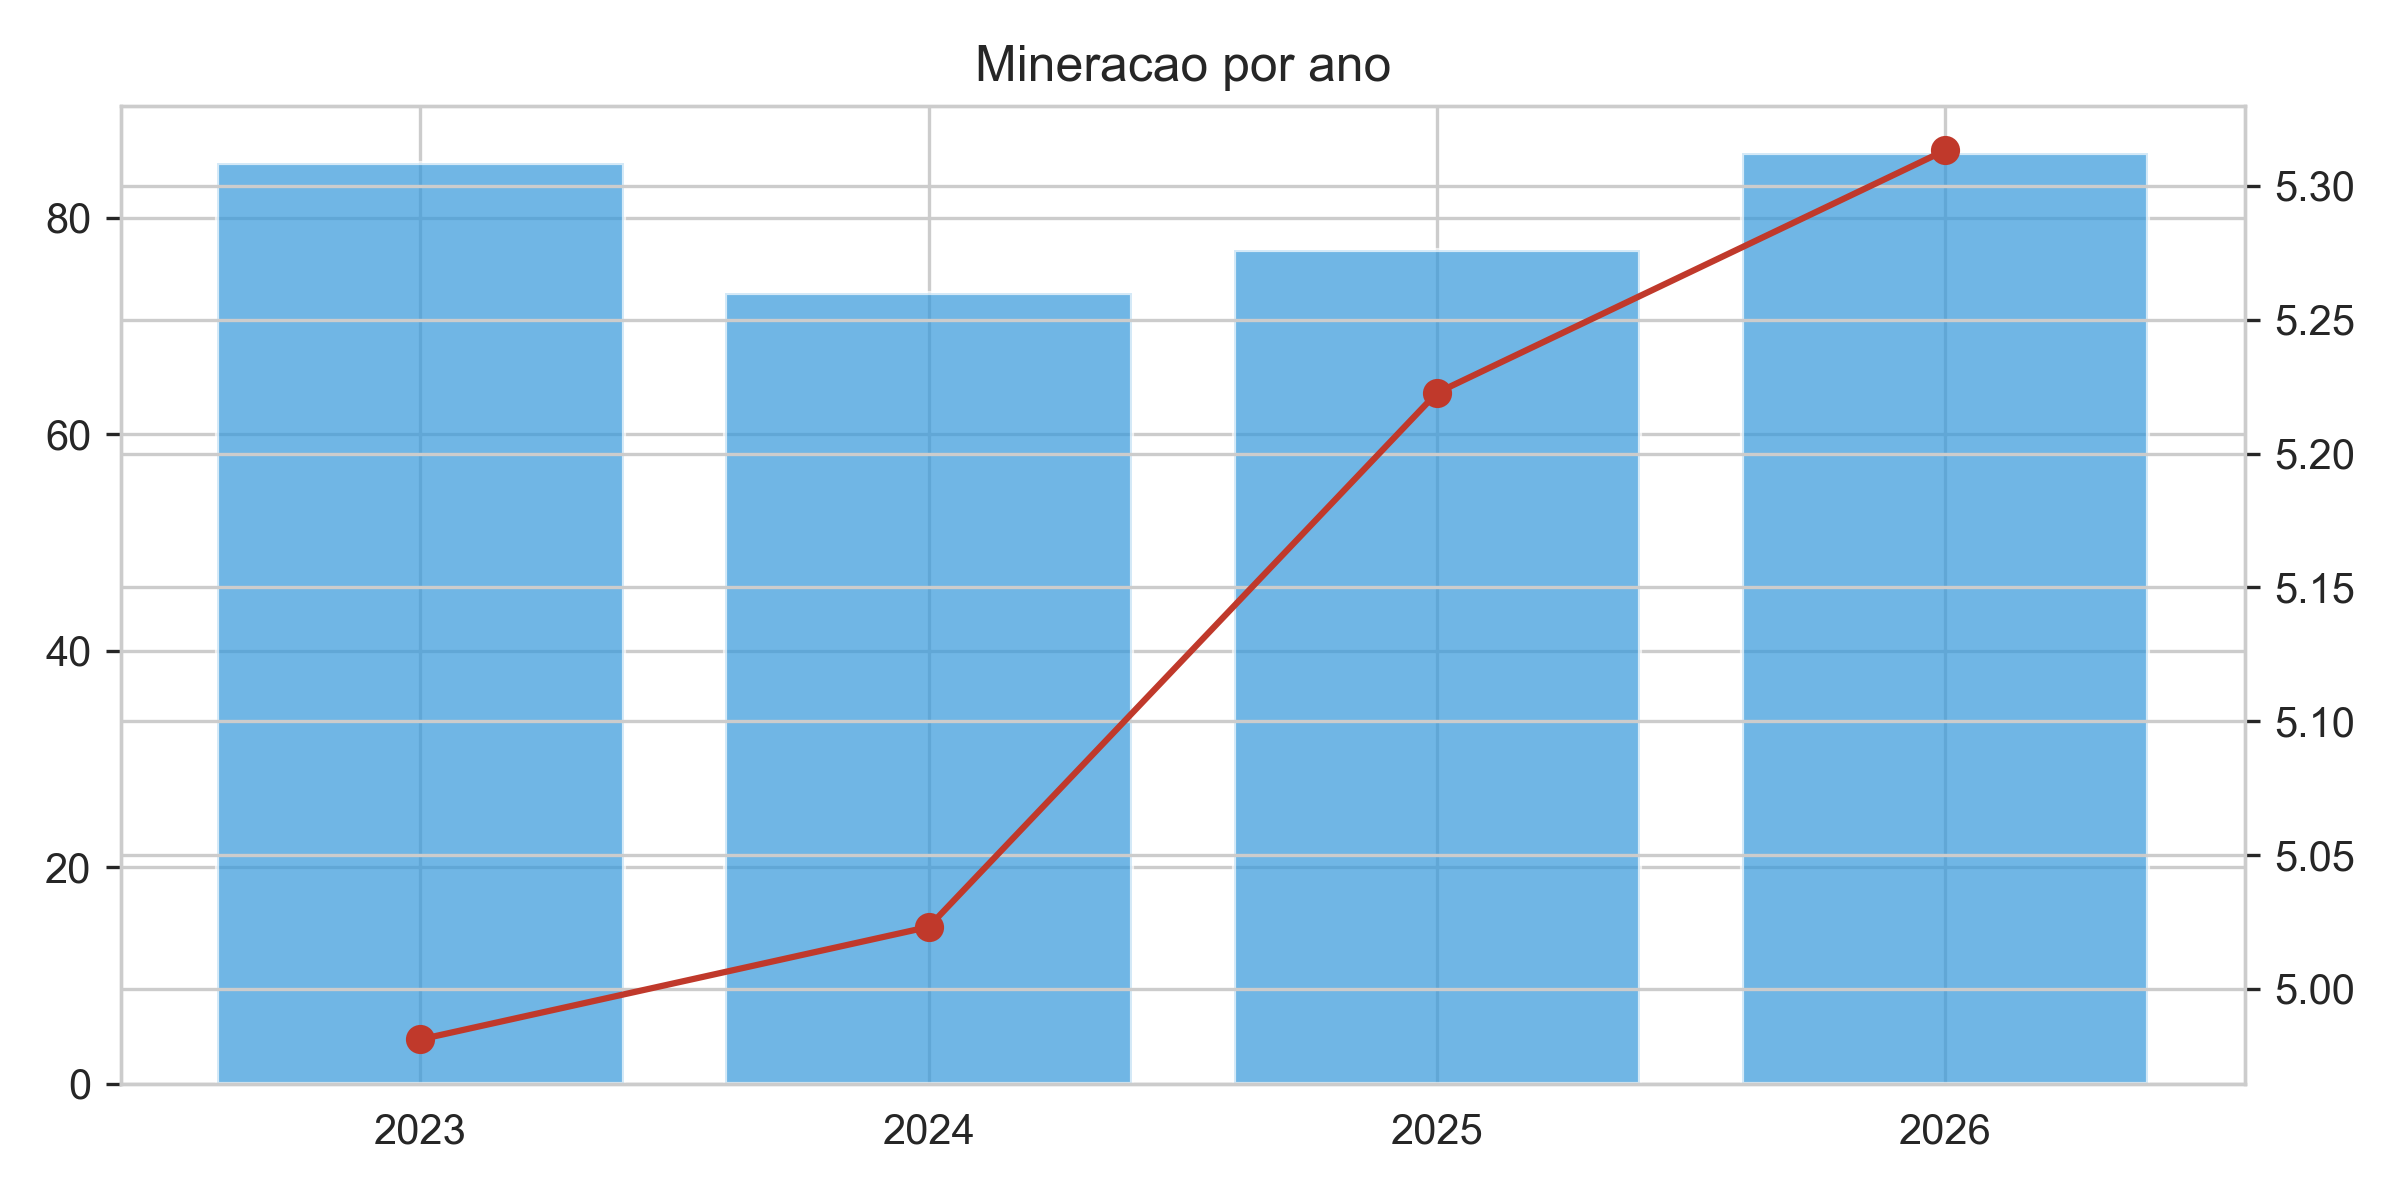
\includegraphics[width=\textwidth]{08_mineracao_por_ano.png}
        \caption{Regras mineradas por ano.}
    \end{subfigure}
    \caption{Resultados da minera\c{c}\~ao FP-Growth restrita.}
    \label{fig:mining}
\end{figure}

\subsection{Estabilidade Temporal e Estratos}

Executamos FP-Growth independentemente por ano (2023--2026) e classificamos regras como \textbf{est\'aveis} quando presentes em $\geq 50\%$ dos anos. Identificamos \textbf{87 regras est\'aveis}, das quais 31 aparecem nos quatro anos (Tabela~\ref{tab:stab}). A regra \{Transitar na contram\~ao, Colis\~ao frontal, Zona Rural\} $\rightarrow$ Fatal permanece est\'avel com lift m\'edio 5,56.

\begin{table}[H]
    \centering
    \caption{Amostra de regras est\'aveis em 4/4 anos.}
    \label{tab:stab}
    \small
    \begin{tabular}{@{}p{6.5cm}rrr@{}}
\toprule
\textbf{Regra (antecedente)} & \textbf{Anos} & \textbf{Conf. (\%)} & \textbf{Lift m\'ed.} \\
\midrule
causa acidente=Transitar na contramão; tipo acidente=Colisão frontal; uso solo=Não & 4/4 & 43,9 & 5,56 \\
causa acidente=Transitar na contramão; tipo acidente=Colisão frontal; tipo pista=Simples & 4/4 & 39,6 & 5,01 \\
fase dia=Plena Noite; tipo acidente=Colisão frontal; uso solo=Não & 4/4 & 39,0 & 4,94 \\
condicao metereologica=Céu Claro; tipo acidente=Colisão frontal; uso solo=Não & 4/4 & 38,2 & 4,85 \\
causa acidente=Transitar na contramão; tipo acidente=Colisão frontal & 4/4 & 37,8 & 4,78 \\
fase dia=Plena Noite; tipo acidente=Atropelamento de Pedestre & 4/4 & 36,8 & 4,66 \\
tipo acidente=Atropelamento de Pedestre; uso solo=Não & 4/4 & 35,6 & 4,53 \\
tipo acidente=Colisão frontal; uso solo=Não & 4/4 & 35,4 & 4,49 \\
\bottomrule
\end{tabular}
\end{table}

A minera\c{c}\~ao por estrato de \textit{uso do solo} (urbano vs.\ rural) revelou \textbf{19} e \textbf{54} regras contextuais, respectivamente, confirmando maior densidade de padr\~oes em trechos rurais (Figura~\ref{fig:estratos}).

\begin{figure}[H]
    \centering
    \begin{subfigure}[b]{0.48\textwidth}
        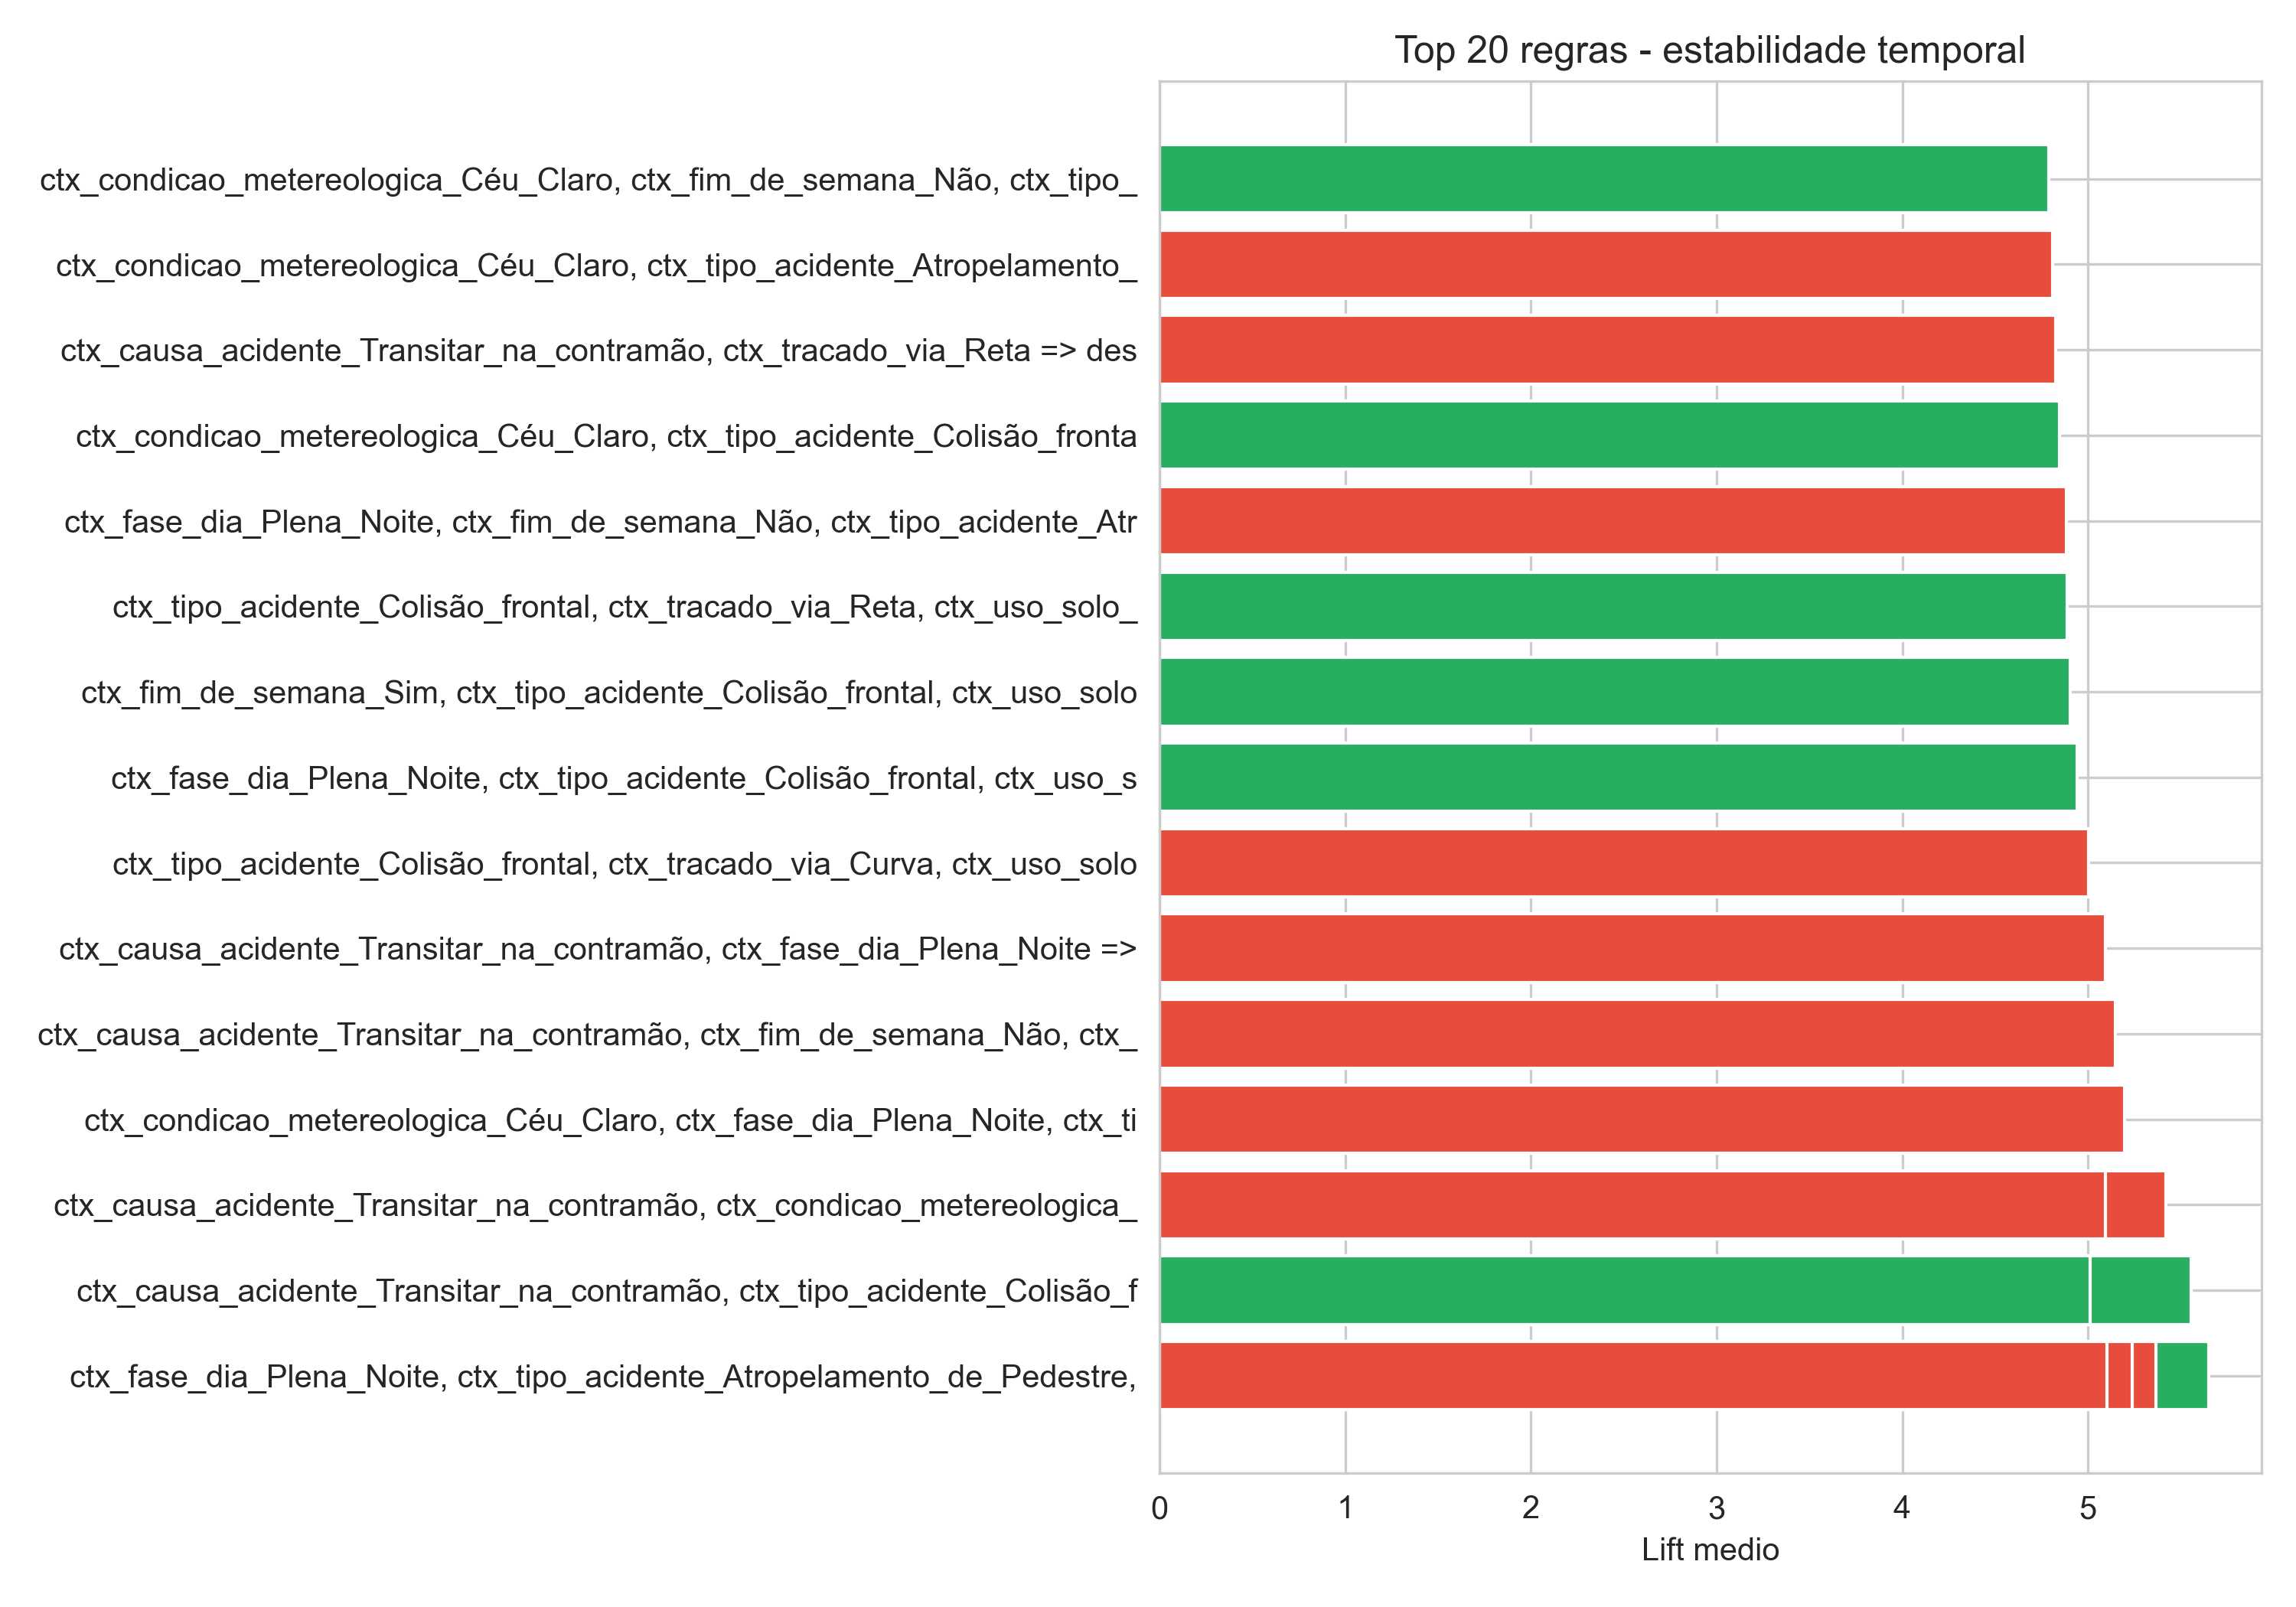
\includegraphics[width=\textwidth]{06_estabilidade_temporal.png}
        \caption{Estabilidade temporal das regras.}
    \end{subfigure}
    \hfill
    \begin{subfigure}[b]{0.48\textwidth}
        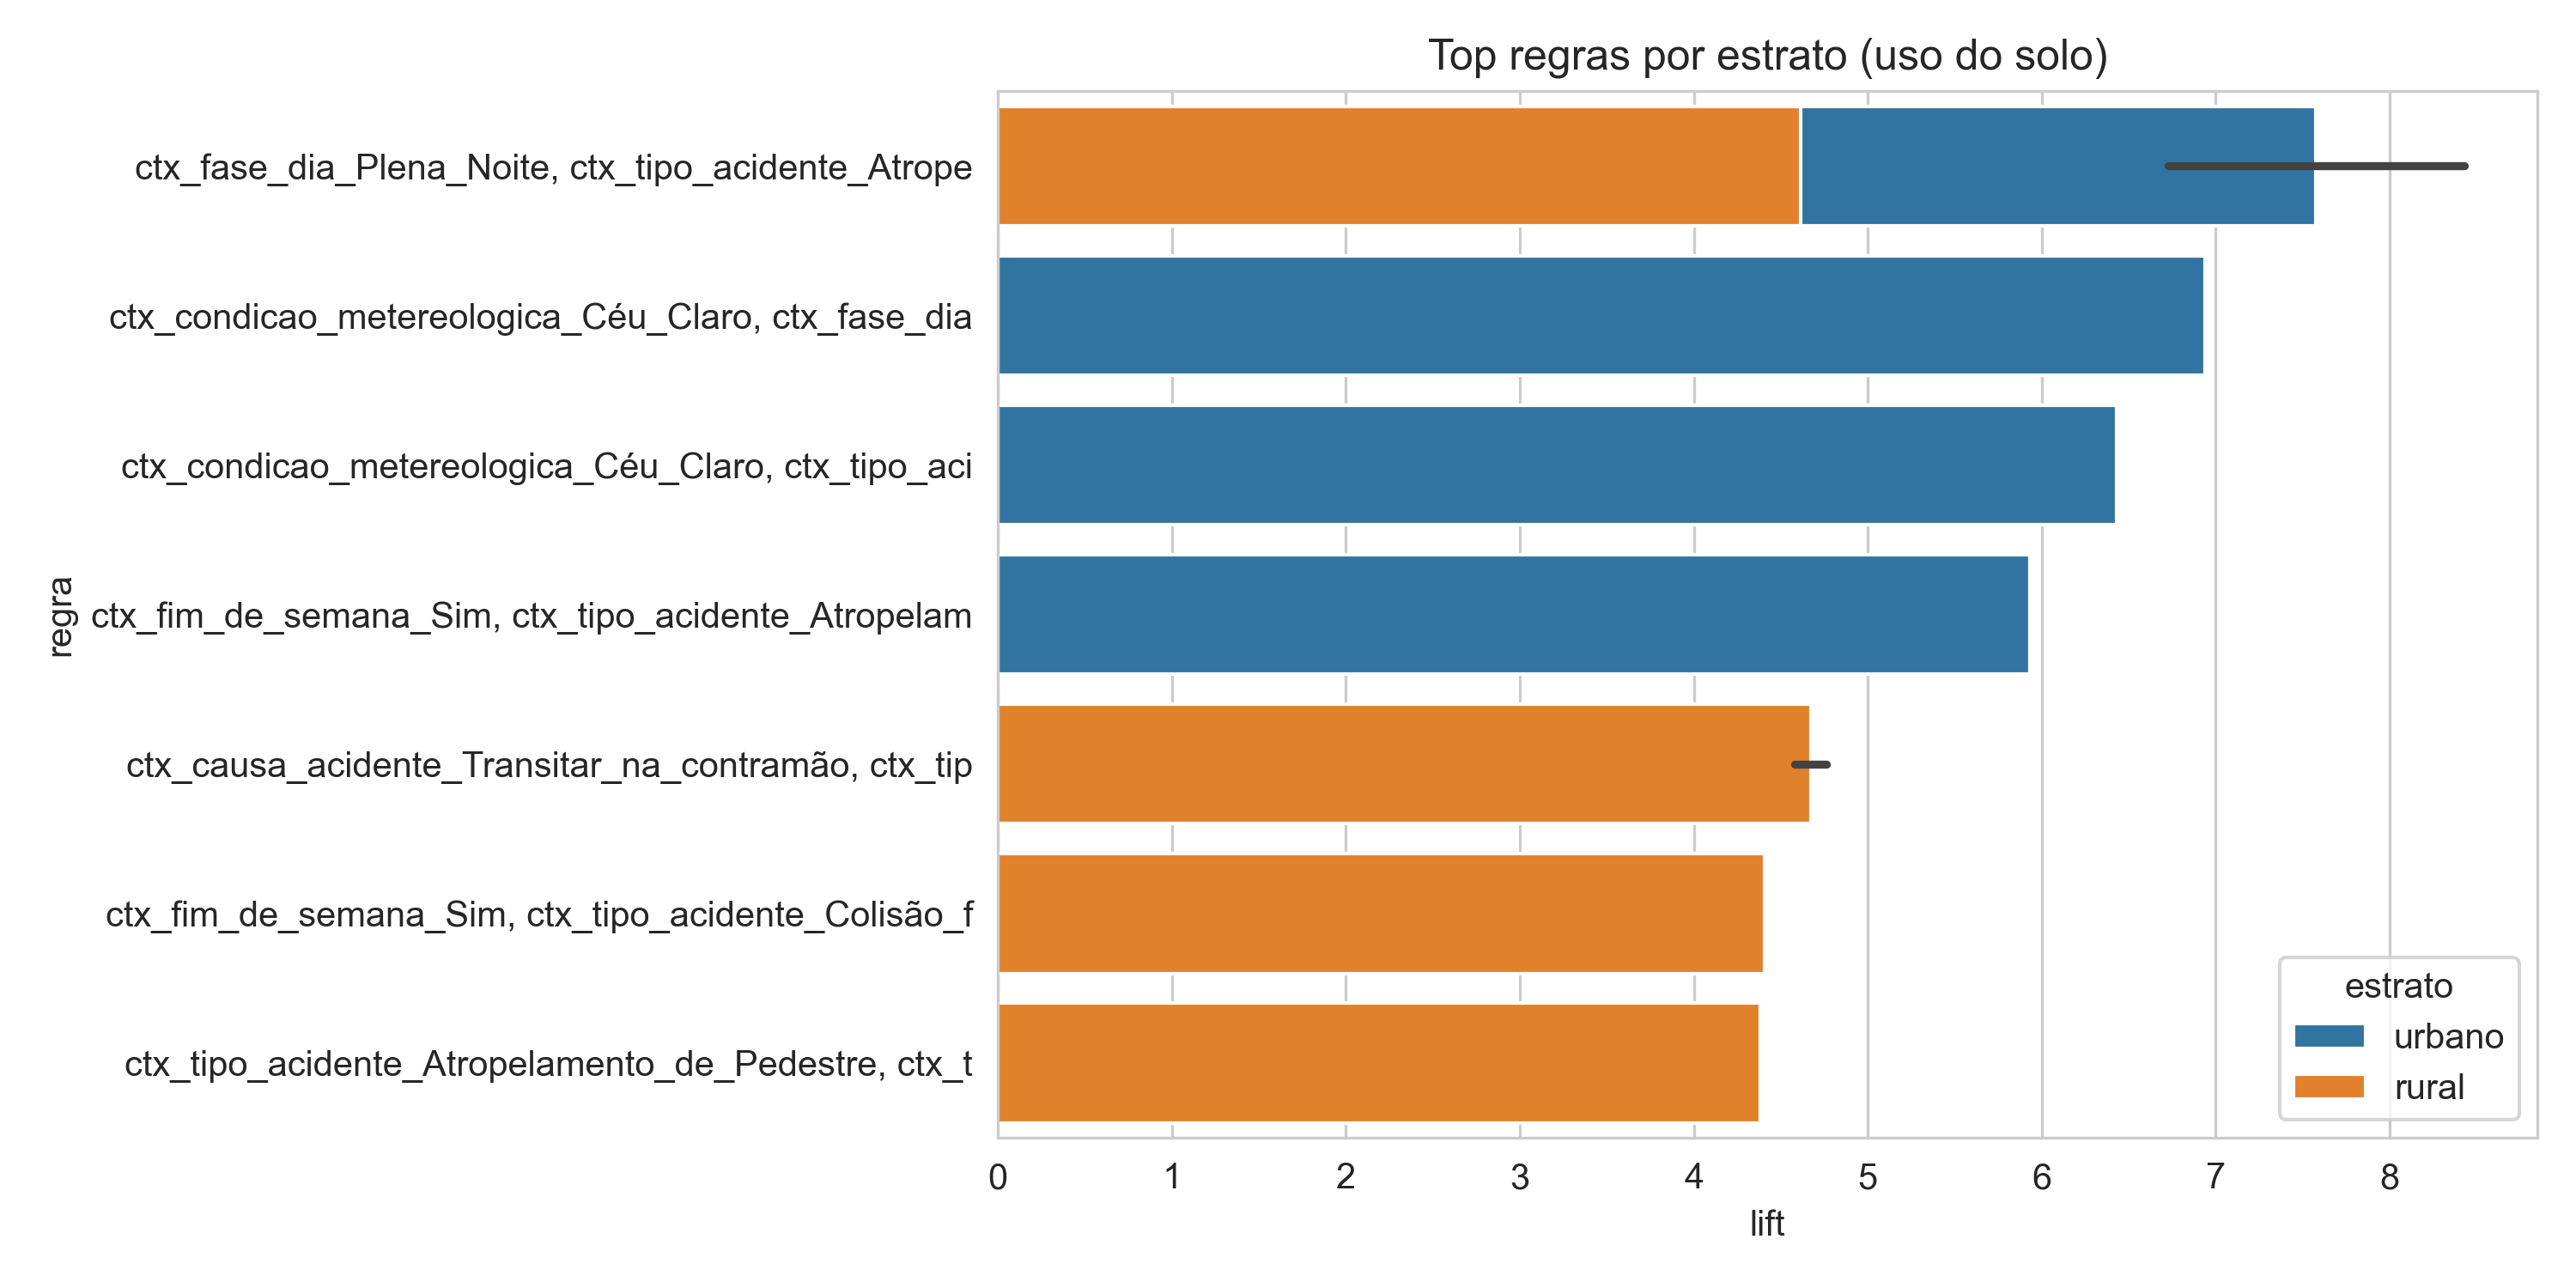
\includegraphics[width=\textwidth]{07_estratos_uso_solo.png}
        \caption{Top regras por estrato (uso do solo).}
    \end{subfigure}
    \caption{Monitoramento temporal e heterogeneidade urbano/rural.}
    \label{fig:estratos}
\end{figure}

\section{An\'alise dos Resultados}

\textbf{H1} (Plena Noite + Pista Simples + Zona Rural): \textbf{parcialmente confirmada}. Regras noturnas em zona rural aparecem entre as de maior lift (Tabela~\ref{tab:top}), embora \textit{pista simples} apare\c{c}a mais frequentemente combinada a colis\~oes frontais do que a atropelamentos.

\textbf{H2} (Finais de semana + Madrugada): \textbf{parcialmente confirmada}. Regras com \texttt{fim\_de\_semana=Sim} e colis\~ao frontal em zona rural apresentam lift 4,76, mas padr\~oes noturnos dominam sobre madrugada isolada.

\textbf{H3} (Colis\~oes frontais e atropelamentos): \textbf{confirmada}. Colis\~ao frontal e atropelamento de pedestre s\~ao os tipos mais recorrentes nos antecedentes de regras de alto lift; transitar na contram\~ao refor\c{c}a colis\~oes frontais fatais (conf.\ $\approx$ 42\%).

\textbf{H4} (Clima adverso): \textbf{refutada parcialmente}. Contrariando a intui\c{c}\~ao, \textit{C\'eu Claro} aparece em regras de alto lift --- poss\'ivel confounding com volume de tr\'afego e visibilidade noturna, n\~ao necessariamente causalidade.

\textbf{H5} (Urbano vs.\ rural): \textbf{confirmada}. Zona rural (\texttt{uso\_solo=N\~ao}) est\'a presente na maioria das regras top e o estrato rural concentra quase tr\^es vezes mais regras que o urbano.

Enfatizamos que todas as regras expressam \textbf{coocorr\^encia estat\'istica}, n\~ao rela\c{c}\~ao causal. Fatores omitidos (velocidade, composi\c{c}\~ao da frota, interven\c{c}\~ao m\'edica) podem explicar parte dos padr\~oes observados.

\section{Diretrizes de IA Respons\'avel}

\subsection{Explicabilidade}

Priorizamos regras com antecedentes curtos ($\leq 3$ itens), traduzidas para linguagem natural (notebook~05 e Tabela~\ref{tab:top}). Removemos redund\^ancias e tautologias (Pacote~A). Cada regra \'e acompanhada de suporte, confian\c{c}a e lift, com disclaimer expl\'icito sobre associa\c{c}\~ao $\neq$ causalidade. \textit{Trade-off}: regras complexas potencialmente relevantes foram descartadas em favor de interpretabilidade.

\subsection{Monitoramento e Avalia\c{c}\~ao}

Executamos FP-Growth por ano e calculamos recorr\^encia temporal (Figura~\ref{fig:estratos}). Regras est\'aveis (87) recebem maior peso anal\'itico; transit\'orias s\~ao interpretadas com cautela. \textit{Trade-off}: subdivis\~ao temporal reduz suporte por janela, dificultando padr\~oes sobre fatais em anos isolados.

\section{Conclus\~oes e Perspectivas}

Este projeto aplicou FP-Growth de forma restrita e interpret\'avel sobre 26.899 acidentes com v\'itimas em MG (2023--2026), produzindo 76 regras contexto $\rightarrow$ Fatal e evid\^encias de estabilidade temporal. Os padr\~oes refor\c{c}am a gravidade de colis\~oes frontais e atropelamentos em trechos rurais e noturnos, subsidiando hip\'oteses para pol\'iticas de preven\c{c}\~ao --- sempre como associa\c{c}\~oes estat\'isticas, n\~ao prescri\c{c}\~oes causais.

Como extens\~oes futuras, sugere-se: (i)~incorporar vari\'aveis veiculares e de infraestrutura adicional; (ii)~comparar com modelos preditivos (classifica\c{c}\~ao) como linha de base; (iii)~expandir o recorte geogr\'afico; e (iv)~integrar dados de interven\c{c}\~ao (tempo de socorro) para reduzir confounding.

\addcontentsline{toc}{section}{Refer\^encias}
\begin{thebibliography}{99}
    \bibitem{agrawal1994} AGRAWAL, R.; SRIKANT, R. Fast algorithms for mining association rules. In: \textit{Proceedings of the 20th International Conference on Very Large Data Bases}, 1994.
    \bibitem{han2000} HAN, J.; PEI, J.; YIN, Y. Mining frequent patterns without candidate generation. \textit{ACM SIGMOD Record}, v.~29, n.~2, p.~1--12, 2000.
    \bibitem{zaki2020} ZAKI, M. J.; MEIRA JR, W. \textit{Data Mining and Machine Learning: Fundamental Concepts and Algorithms}. 2nd ed. Cambridge University Press, 2020.
    \bibitem{wirth2000} WIRTH, R.; HIPP, J. CRISP-DM: Towards a standard process model for data mining. In: \textit{Proceedings of the 4th International Conference on the Practical Applications of Knowledge Discovery and Data Mining}, 2000.
    \bibitem{tan2006} TAN, P.-N.; STEINBACH, M.; KUMAR, V. \textit{Introduction to Data Mining}. Addison-Wesley, 2006.
    \bibitem{prf2026} BRASIL. Pol\'icia Rodovi\'aria Federal. \textbf{Dados Abertos da PRF}. Bras\'ilia, 2026. Dispon\'ivel em: \url{https://www.gov.br/prf/pt-br/acesso-a-informacao/dados-abertos/dados-abertos-da-prf}.
\end{thebibliography}

\end{document}
